% Created 2018-12-13 Thu 23:54
% Intended LaTeX compiler: pdflatex
\documentclass[11pt]{article}
\usepackage[utf8]{inputenc}
\usepackage[T1]{fontenc}
\usepackage{graphicx}
\usepackage{grffile}
\usepackage{longtable}
\usepackage{wrapfig}
\usepackage{rotating}
\usepackage[normalem]{ulem}
\usepackage{amsmath}
\usepackage{textcomp}
\usepackage{amssymb}
\usepackage{capt-of}
\usepackage{hyperref}
\usepackage{minted}
\author{Anoop G R}
\date{\today}
\title{}
\hypersetup{
 pdfauthor={Anoop G R},
 pdftitle={},
 pdfkeywords={},
 pdfsubject={},
 pdfcreator={Emacs 26.1 (Org mode 9.1.9)}, 
 pdflang={English}}
\begin{document}

\tableofcontents


\section{Anoop index:}
\label{sec:org60c6138}
How Do I Get Started?
Applied Machine Learning Process
Linear Algebra
Statistical Methods
Understand Machine Learning Algorithms
Python Machine Learning (scikit-learn)
Code Algorithm from Scratch (Python)
Introduction to Time Series Forecasting (Python)
XGBoost in Python (Stochastic Gradient Boosting)
Deep Learning (Keras)
Long Short-Term Memory (LSTM)
Deep Learning for Natural Language Processing (NLP)
Deep Learning for Time Series Forecasting


\section{experimental0}
\label{sec:org462f6c1}
chrome history suggestions based on a neural network
read to get ideas for projects: \url{https://machinelearningmastery.com/self-study-machine-learning-projects/}
maintain a ml daily blog?
how to get computers to talk to each other using socket programming
use free time with phone to study google maps of Bangalore like guttapalli
buy toothbrush, bigger bulb for room
sabji kitne ki hai app

\section{How Do I Get Started?}
\label{sec:org336bba8}

\subsection{articles-read, worth rereading}
\label{sec:org4b43a9e}
$$ Applied Machine Learning Process
 $$ Intermediate: Python Ecosystem.

\$\$ Step 4: Practice on Datasets. Select datasets to work on and practice the process. 

$$ Practice Machine Learning with Small In-Memory Datasets
 $$ Tour of Real-World Machine Learning Problems
\$\$ Work on Machine Learning Problems That Matter To You

\$\$ Step 5: Build a Portfolio. Gather results and demonstrate your skills. 

$$ Build a Machine Learning Portfolio
 $$ Get Paid To Apply Machine Learning
\$\$ Machine Learning For Money

For more on this top-down approach, see:

$$ The Machine Learning Mastery Method
$$ Machine Learning for Programmers

Many of my students have used this approach to go on and do well in Kaggle competitions and get jobs as Machine Learning Engineers and Data Scientists.

\subsection{notes}
\label{sec:org2f6b6a8}

\subsubsection{intro}
\label{sec:org5e9fe48}
sckit-learn is higher level than numpy \& scipy
machine learning is a subset of artificial intelligence
artificial learning is a more consistent name for machine learning

\subsubsection{some key word definitions:}
\label{sec:org5135a72}
Model: A machine learning model can be a mathematical representation
of a real-world process. To generate a machine learning model you will
need to provide training data to a machine learning algorithm to learn
from.

Algorithm: Machine Learning algorithm is the hypothesis set that is
taken at the beginning before the training starts with real-world
data. When we say Linear Regression algorithm, it means a set of
functions that define similar characteristics as defined by Linear
Regression and from those set of functions we will choose one function
that fits the most by the training data.

Training: While training for machine learning, you pass an algorithm
with training data. The learning algorithm finds patterns in the
training data such that the input parameters correspond to the target.
The output of the training process is a machine learning model which
you can then use to make predictions. This process is also called
“learning”.

Regression: Regression techniques are used when the output is
real-valued based on continuous variables. For example, any time
series data. This technique involves fitting a line.

Classification: In classification, you will need to categorize data
into predefined classes. For example, an email can either be ‘spam’ or
‘not spam’.

Target: The target is whatever the output of the input variables. It
could be the individual classes that the input variables maybe mapped
to in case of a classification problem or the output value range in a
regression problem. If the training set is considered then the target
is the training output values that will be considered.

Feature: Features are individual independent variables that act as the
input in your system. Prediction models use features to make
predictions. New features can also be obtained from old features using
a method known as ‘feature engineering’. More simply, you can consider
one column of your data set to be one feature. Sometimes these are
also called attributes. And the number of features are called
dimensions.

Label: Labels are the final output. You can also consider the output
classes to be the labels. When data scientists speak of labeled data,
they mean groups of samples that have been tagged to one or more
labels.

Overfitting: An important consideration in machine learning is how
well the approximation of the target function that has been trained
using training data, generalizes to new data. Generalization works
best if the signal or the sample that is used as the training data has
a high signal to noise ratio. If that is not the case, generalization
would be poor and we will not get good predictions. A model is
overfitting if it fits the training data too well and there is a poor
generalization of new data.

Regularization: Regularization is the method to estimate a preferred
complexity of the machine learning model so that the model generalizes
and the over-fit/under-fit problem is avoided. This is done by adding
a penalty on the different parameters of the model thereby reducing
the freedom of the model.

Parameter and Hyper-Parameter: Parameters are configuration variables
that can be thought to be internal to the model as they can be
estimated from the training data. Algorithms have mechanisms to
optimize parameters. On the other hand, hyperparameters cannot be
estimated from the training data. Hyperparameters of a model are set
and tuned depending on a combination of some heuristics and the
experience and domain knowledge of the data scientist.


\section{\url{https://machinelearningmastery.com/python-machine-learning-mini-course/}}
\label{sec:org8b26e2c}
14Lessons
\subsection{pre requisite \url{https://machinelearningmastery.com/gentle-introduction-to-the-bias-variance-trade-off-in-machine-learning/}}
\label{sec:org492cc74}
\textbf{Bias Error}
Bias are the simplifying assumptions made by a model to make the target function easier to learn.
Low Bias: Suggests less assumptions about the form of the target function.
High-Bias: Suggests more assumptions about the form of the target function.

Examples of low-bias machine learning algorithms include: Decision Trees, k-Nearest Neighbors and Support Vector Machines.
Examples of high-bias machine learning algorithms include: Linear Regression, Linear Discriminant Analysis and Logistic Regression.

\textbf{Variance Error}
Variance is the amount that the estimate of the target function will change if different training data was used.

Examples of low-variance machine learning algorithms include: Linear Regression, Linear Discriminant Analysis and Logistic Regression.
Examples of high-variance machine learning algorithms include: Decision Trees, k-Nearest Neighbors and Support Vector Machines.

Fig 1. bulls-eye visualise \url{http://scott.fortmann-roe.com/docs/BiasVariance.html}

skill of the model, a score with 
a high variance = (that may change a lot based on the data used to fit the model), or 
a high bias = (such as an overestimate of the skill of the model).

\subsection{1 - install}
\label{sec:orgaecae8c}
\subsubsection{next time try using this tutorial \url{https://sourabhbajaj.com/mac-setup/Python/numpy.html}}
\label{sec:orgb199b74}
\subsubsection{make a new virtualenv}
\label{sec:orgfb5f7f6}
\begin{minted}[]{shell}
pwd
\end{minted}


Use :session: property to speed up org-babel when possible to use the same session
\begin{minted}[]{bash}
source ~/.bashrc
#mkvirtualenv mlm
workon mlm
which python
\end{minted}

\begin{minted}[]{elisp}
(pyvenv-workon "mlm2")
\end{minted}

\subsubsection{install \url{https://stackoverflow.com/questions/26319762/how-to-install-scipy-stack-with-pip-and-homebrew}}
\label{sec:orge42f5a3}
pip install numpy
brew install gcc
pip install scipy
brew install freetype
pip install matplotlib
pip install nose
pip install pandas
pip install sympy
pip install ipython[all]
brew install pyqt
brew install qt
brew install sip
\#after this edit the 2 scripts
\subsubsection{check if properly isntalled using .\_\(_{\text{version}}\) \_ after import}
\label{sec:orgc8aaeaa}

using python snippets inside orgmode \url{https://orgmode.org/worg/org-contrib/babel/languages/ob-doc-python.html}
installed python-mode from package-list-packages for emacs
\begin{minted}[]{common-lisp}
(pyvenv-workon "mlm")
\end{minted}

Fixed some errors using: pip install nose pyparsing python-dateutil pep8
\begin{minted}[]{python}
import sys
import scipy
import numpy
import matplotlib
import pandas
import sklearn

print(f'python: {sys.version}')
print(f'scipy: {scipy.__version__}')
print(f'numpy: {numpy.__version__}')
print(f'matplotlib {matplotlib.__version__}')
print(f'pandas {pandas.__version__}')
print(f'sklearn {sklearn.__version__}')

\end{minted}

\subsection{2 - python, pandas, numpy, mathplotlib veeery basics}
\label{sec:org48e0601}

\subsubsection{python, also refer in-y-minutes file for future reference}
\label{sec:orgb17536d}
\begin{minted}[]{python}
if 1>2:
    print("wtf")
else:
    print("ok")

try:
    # Use "raise" to raise an error
    raise IndexError("This is an index error")
except IndexError as e:
    print("its indexerror")
    pass                 # Pass is just a no-op. Usually you would do recovery here.
except (TypeError, NameError):
    print("its typeerror or nameerror")
    pass                 # Multiple exceptions can be handled together, if required.
else:                    # Optional clause to the try/except block. Must follow all except blocks
    print("All good!")   # Runs only if the code in try raises no exceptions
finally:                 #  Execute under all circumstances
    print("We can clean up resources here")
\end{minted}

\begin{minted}[]{python}
def accepts_variable_number_of_arguments(*args):
    print(type(args))
    print(args)

accepts_variable_number_of_arguments(1,2,3)

def accepts_variable_number_of_keyword_arguments(**kwargs):
    print(type(kwargs))
    print(kwargs)

accepts_variable_number_of_keyword_arguments(name="anoop", work="code")

def accepts_both_args_and_kwargs(*args, **kwargs):
    print(args)
    print("------")
    print(kwargs)

accepts_both_args_and_kwargs(1,2,3,a="4",b="5",last0="6")
\end{minted}

\subsubsection{numpy basics}
\label{sec:orgef175d3}

\begin{center}
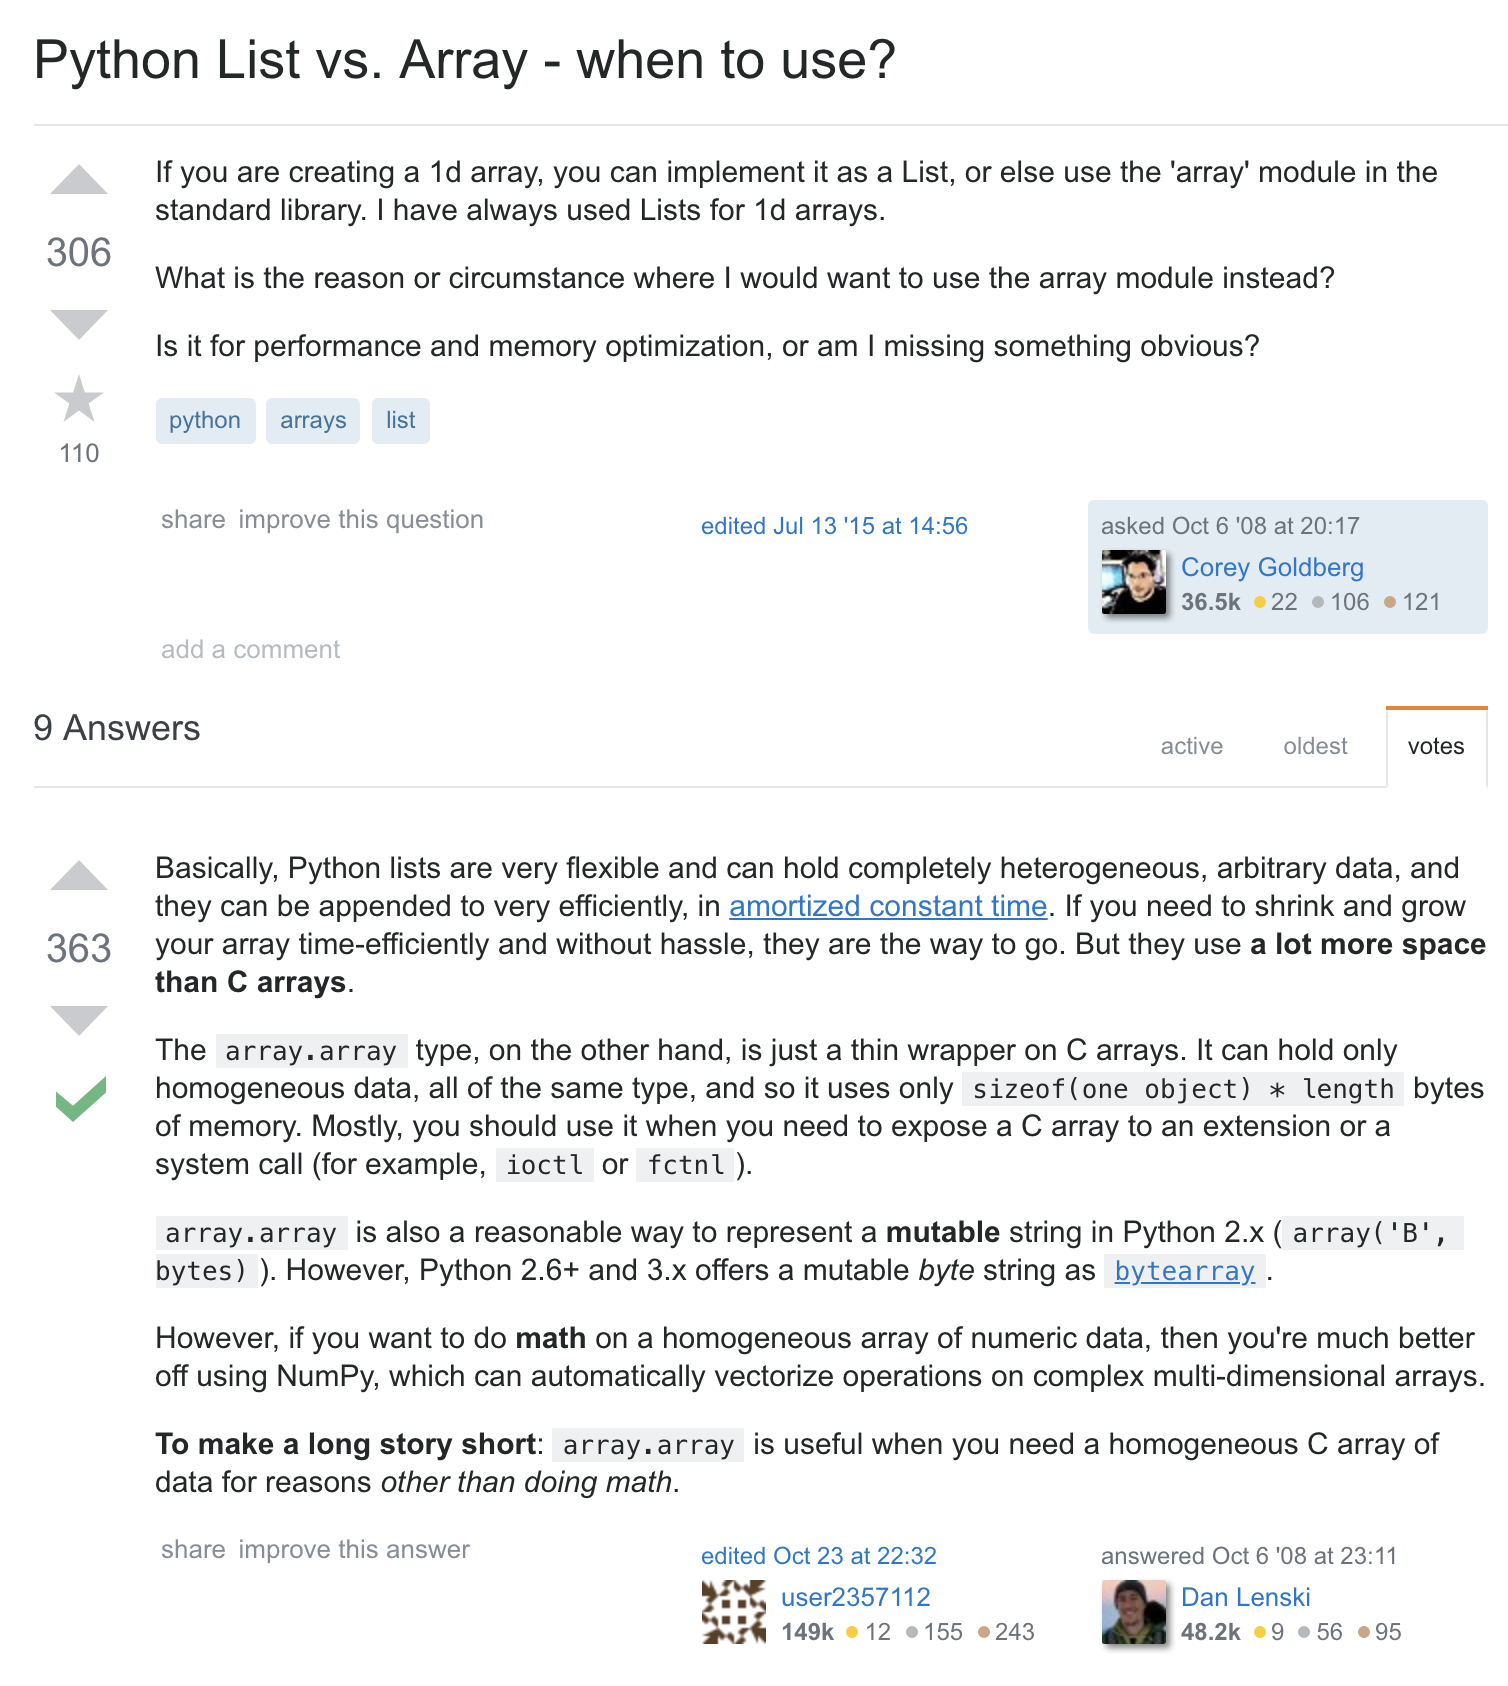
\includegraphics[width=.9\linewidth]{screenshots0/Screenshot 2018-12-11 at 5.16.28 PM.png}
\end{center}

\textbf{numpy official tutorial}
\url{https://docs.scipy.org/doc/numpy-1.15.0/user/quickstart.html}
\begin{minted}[]{python}
  import numpy as np
  a = np.arange(15).reshape(3,5)
  print(a)
  a.shape
  a.ndim
  a.dtype.name
  #dir(a)
  a.size
  type(a)
  b = np.array([6,7,8])
  b
  type(b)

  np.zeros([2,3])
  np.arange(15)
  np.linspace(0,9, 19)

  from numpy import pi
  x = np.linspace(0, 2*pi, 5)
  np.sin(x)
  #2 decimal places
  np.around(np.sin(x), decimals=2)

  A = np.array([[1,2],[3,4]])
  I = np.array([[1,0],[0,1]])
  elementwise = A * I
  matrix_product = A @ I
  print(elementwise, "\n", matrix_product)

  a = np.ones(3, dtype=np.int32)
  b = np.linspace(0, 1, 3)
  c = a + b
  print(a,b,c)
  c.dtype.name
  c*1j
  np.ones(1)
  my_e = np.exp(np.ones(1))
  from numpy import e
  e
  print(e, my_e)
  d = np.exp(c*1j)
  d.dtype
  # exp, sin etc are called numpy universal functions

  # multidimensional array
c = np.array([
    [
	[  0,  1,  2],
	[ 10, 12, 13]
    ],
    [
	[100,101,102],
	[110,112,113]
    ]
])
c.shape
# Visualize0 2,2,3 as you traverse from the topmost bracket to the inner ones
for i in c.flat:
    print(i, end=" // ")
print("\n")
id(c) #id is unique identifier of an object in python


\end{minted}

axis in numpy

\href{screenshots0/Screenshot\%202018-12-11\%20at\%206.06.43\%20PM.png}{file:\textasciitilde{}/ml/flipshope/screenshots0/Screenshot 2018-12-11 at 6.06.43 PM.png}

matplotlib python is not installed as a framework error, solution:
\url{https://stackoverflow.com/questions/34977388/matplotlib-runtimeerror-python-is-not-installed-as-a-framework}

Above is a hacky solution
I need to switch away from virtualenv \& virtualenvwrapper and move to venv entirely
Also, reddit recommends to avoid the pyenv or any wrapper around venv \&\& strongly recommends to use venv directly
venv ships by default with python >= 3.3
\url{https://matplotlib.org/faq/osx\_framework.html}
\url{https://news.ycombinator.com/item?id=18612590}
\url{https://news.ycombinator.com/item?id=18247512}
:) 	
andybak 54 days ago [-]
In case this scares any new users, I've used nothing more than pip and virtualenv for several years with no issues of note.



\begin{minted}[]{python}
import numpy as np
import matplotlib.pyplot as plt
#import matplotlib  
#matplotlib.use('TkAgg')   
#import matplotlib.pyplot as plt 

def mandelbrot( h,w, maxit=20 ):
    """Returns an image of the Mandelbrot fractal of size (h,w)."""
    y,x = np.ogrid[ -1.4:1.4:h*1j, -2:0.8:w*1j ]
    c = x+y*1j
    z = c
    divtime = maxit + np.zeros(z.shape, dtype=int)

    for i in range(maxit):
	z = z**2 + c
	diverge = z*np.conj(z) > 2**2            # who is diverging
	div_now = diverge & (divtime==maxit)  # who is diverging now
	divtime[div_now] = i                  # note when
	z[diverge] = 2                        # avoid diverging too much

    return divtime
plt.imshow(mandelbrot(400,400))
plt.show()
\end{minted}

\begin{minted}[]{python}
import sys
print(sys.path)
\end{minted}

\textbf{real-python tutorial}
\url{https://realpython.com/numpy-array-programming/}

When it comes to computation, there are really three concepts that lend NumPy its power:
Vectorization
Broadcasting
Indexing

\begin{minted}[]{python}
import numpy as np

arr = np.arange(36).reshape(3,4,3)
arr

"""
visualize0:-

00 01 02 03 04 05 06 07 08 09 10 11 
12 13 14 15 16 17 18 19 20 21 22 23 
24 25 26 27 28 29 30 31 32 33 34 35 

00 01 02 
03 04 05 
06 07 08 
09 10 11 

[#3 items
[#4 items
[]
[]
[]
[]
]...
]
"""
a = np.array([2,3,4])
b = 2
b_broadcasted = np.broadcast(a,b)
print(list(b_broadcasted))
# rest of this tutorial seemed a bit advanced, skip for now, come back later

\end{minted}

\textbf{Note} Pandas is a library built on top of NumPy

todo: switch to jupyter notebook instead of emacs: 
\url{https://github.com/millejoh/emacs-ipython-notebook}
\url{http://millejoh.github.io/emacs-ipython-notebook/}
\url{https://www.youtube.com/watch?v=wtVF5cMhBjg}
\url{https://news.ycombinator.com/item?id=9728143}
\url{https://github.com/gregsexton/ob-ipython}

\subsubsection{matplotlib basics}
\label{sec:org531a9f5}
matplotlib, is written in pure Python and is heavily dependent on NumPy

Matplotlib is conceptually divided into three parts:
pylab interface (similar to MATLAB) – pylab tutorial, this is the matplotlib.pyplot import
Matplotlib frontend or API – artist tutorial
backends – drawing devices or renderers

Lets learn pyplot
\url{https://matplotlib.org/users/pyplot\_tutorial.html\#pyplot-tutorial}

venv basics to switch from virtualenv

python3 -m venv mlm2
source mlm2/bin/activate

pyvenv-deactivate

\begin{minted}[]{python}
import matplotlib
#matplotlib.use('MacOSX')
import matplotlib.pyplot as plt

plt.plot([0, 1, 4, 9, 16])
#plt.show()

plt.plot([0, 1, 4, 9, 16], 'ro')
#plt.show()

plt.plot([0.5], 'y.')
plt.show()
\end{minted}

\subsubsection{Pandas -basics:}
\label{sec:orgeb9db5b}
Todo:\url{https://pandas.pydata.org/pandas-docs/stable/dsintro.html\#dsintro}
Todo:Official beginner tutorial: \url{https://pandas.pydata.org/pandas-docs/stable/10min.html}
Todo: Intermediate - Julia Evans - \url{https://jvns.ca/blog/2013/12/22/cooking-with-pandas/}
"take a real dataset or three, play around with it, and learn how to use pandas along the way."


Panda Series \& DataFrames:
\url{https://medium.freecodecamp.org/series-and-dataframe-in-python-a800b098f68}
\begin{minted}[]{python}
#Series and DataFrames
import pandas as pd
x1 = pd.Series([6,3,4,6])
x = pd.Series([6,3,4,6], index=['a','b','c','d'])
x
y = pd.Series(3, index=['a', 'b', 'c', 'd'])
y

#DataFrames
import numpy as np
dates = pd.date_range('20181201', periods = 8)

my_narray = np.random.randn(8,3)
list('ABC')

df = pd.DataFrame(index = dates, data = my_narray, columns = ['A','B','C'])
df_absolute = df.apply(abs)
\end{minted}

So pandas is kinda like an excel sheet0

\begin{minted}[]{python}
import numpy as np

np.arange(4)
ma = np.arange(4).reshape((2,2))

import pandas

p = pandas.DataFrame(ma)

print(ma[1,0])
print(p[1])
print(p[1][0] == ma[1][0])
print(p.shape)


\end{minted}

\subsection{3 - Load csv}
\label{sec:orgcd7a4cc}
\url{https://realpython.com/python-csv/}
\url{https://github.com/jbrownlee/Datasets}

\textbf{Work with csv using python's csv module}
\begin{minted}[]{python}
import csv

with open('iris.csv') as csv_file:
    """
    for line in csv_file:
	print(line)
	pass
    """
    csv_reader = csv.reader(csv_file)
    for line in csv_reader:
	#print(line)
	pass

my_fieldnames = ("sepal_length", "sepal_width", "petal_length", "petal_width", "class")

with open('iris.csv') as csv_file:
    csv_dict_reader = csv.DictReader(csv_file, fieldnames=my_fieldnames)
    for line in csv_dict_reader:
	#print(line)
	pass

with open('test_writeout.csv', mode='w') as out_file:
    csv_writer = csv.writer(out_file)
    csv_writer.writerow(["row", "1"])
    csv_writer.writerow(["row", "2"])
    #
    csv_dict_writer = csv.DictWriter(out_file, fieldnames = my_fieldnames)
    csv_dict_writer.writeheader()
    csv_dict_writer.writerow({"sepal_length": 1, "sepal_width": 2, "petal_length": 3, "petal_width": 4, "class": 5})


\end{minted}

\textbf{Work with csv using numpy}
\begin{minted}[]{python}
import numpy as np

with open("numpy_loadtxt_input.txt") as input_file:
    """
    for line in input_file:
	print(line)
    """
    my_nparray = np.loadtxt(input_file, delimiter=" ")
    print(my_nparray)
    print(my_nparray.dtype)
\end{minted}

\textbf{Work with csv usign pandas}
\begin{minted}[]{python}
import pandas
df = pandas.read_csv('pandas_read_csv.csv')
print(df)

df2 = pandas.read_csv('pandas_read_csv.csv', parse_dates=['Hire Date'], index_col='Name')
print(df2)

my_col_names = ("Name", "Hired_on", "Salary", "sick_days_remaining")
df3 = pandas.read_csv('pandas_read_csv.csv', header=None, names=my_col_names,
parse_dates=['Hired_on'])
print(df3)

df3.to_csv('pandas_to_csv.csv')
\end{minted}


\subsection{4 - use pandas.DataFrame helper functions to describe data with statistics}
\label{sec:orgb13fc12}
\begin{minted}[]{python}
# Scatter Plot Matrix
import matplotlib.pyplot as plt
import pandas

my_col_names = ("num_preg", "plasma_glucose", "blood_pressure", "triceps_skin_thickness", "serum_insulin", "bmi", "diabetes_pedigree", "age", "class")
df = pandas.read_csv("https://raw.githubusercontent.com/jbrownlee/Datasets/master/pima-indians-diabetes.data.csv", header=None, names=my_col_names)
#print(df)

from pandas.plotting import scatter_matrix

scatter_matrix(df)
plt.show()

df.corr()
\end{minted}
\subsection{5 - Basic Data Visualization}
\label{sec:org25875c1}
Using pandas and matplotlib together
\begin{minted}[]{python}
# Scatter Plot Matrix
import matplotlib.pyplot as plt
import pandas

my_fieldnames = ("sepal_length", "sepal_width", "petal_length", "petal_width", "class")
data = pandas.read_csv('iris.csv', names=my_fieldnames)
#print(data)

se = data.loc[data["class"] == "Iris-setosa"]
ve = data.loc[data["class"] == "Iris-versicolor"]
vi = data.loc[data["class"] == "Iris-virginica"]

#se.hist()
#ve.hist()
#vi.hist()

se.plot(kind="box")

from pandas.plotting import scatter_matrix
#scatter_matrix(se)

plt.savefig("img/lesson5.png")
return "img/lesson5.png"
\end{minted}


\subsection{6 - Preprocessing data}
\label{sec:org795ea72}

Standardize numerical data (e.g. mean of 0 and standard deviation of 1) using the scale and center options.

Simple example:
\begin{minted}[]{python}
import numpy
narray = numpy.arange(0,4).reshape(2,2)

import pandas
df = pandas.DataFrame(narray, columns=("c1", "c2"))

from sklearn.preprocessing import StandardScaler
scaler = StandardScaler()
scaler.fit(df) #calculates and store mean & standard-deviation for each column

print(scaler.transform(df))
type(scaler.transform(df))
df_standardized = pandas.DataFrame(scaler.transform(df))
\end{minted}

Complex example:
\begin{minted}[]{python}
import matplotlib.pyplot as plt
import pandas

#df is my short for DataFrame
my_col_names = ("num_preg", "plasma_glucose", "blood_pressure", "triceps_skin_thickness", "serum_insulin", "bmi", "diabetes_pedigree", "age", "class")
df = pandas.read_csv("https://raw.githubusercontent.com/jbrownlee/Datasets/master/pima-indians-diabetes.data.csv", header=None, names=my_col_names)
#print(df)

import numpy
array = df.values

X = array[:, :-1]
Y = array[:, -1:]

from sklearn.preprocessing import StandardScaler
scaler = StandardScaler().fit(X)
X_standardized = scaler.transform(X)

#printout
numpy.set_printoptions(precision=2)
print(X_standardized)

df_standardized = pandas.DataFrame(X_standardized)
df_standardized.describe() #you can see that mean=0, sdev=1 for each column

\end{minted}


\subsubsection{skip for now, come back later}
\label{sec:org48c78c5}
Normalize numerical data (e.g. to a range of 0-1) using the range option.
Explore more advanced feature engineering such as Binarizing.

\subsection{7 - Resampling}
\label{sec:org905b12a}
statistical methods called resampling methods are used to split your training
dataset up into subsets, some are used to train the model and others
are held back and used to estimate the accuracy of the model on
unseen data.

\subsection{Google Developers intro to ml}
\label{sec:org6617687}
complete google developers course, its a pre-requisite for this lesson as per me
\url{https://www.youtube.com/playlist?list=PLOU2XLYxmsIIuiBfYad6rFYQU\_jL2ryal}

\subsubsection{1 hello apple or orange using decision tree}
\label{sec:orga541a96}
\begin{minted}[]{python}
from sklearn import tree
features_original = [[140, "smooth"], [130, "smooth"], [150, "bumpy"], [170, "bumpy"]] #weight, texture of fruit
labels_original = ["apple", "apple", "orange", "orange"]

#smooth=1 // bumpy=0
#orange=1 // apple=0
features = [[140, 1], [130, 1], [150, 0], [170, 0]] #weight, texture of fruit
labels = [0, 0, 1, 1]

#train a classifier: 
clf = tree.DecisionTreeClassifier() #instantiate an empty box of rules
clf = clf.fit(features, labels) #learning algorithm fills the above box with rules

#print(clf.predict([[150,0]]))
print(clf.predict([[200,0]]))
\end{minted}


\subsubsection{2 Decision Tree visualization}
\label{sec:orga0543d8}

\begin{minted}[]{python}
from sklearn.datasets import load_iris
from sklearn import tree
iris = load_iris()
print(dir(iris))

print(iris.feature_names) #in this example data_names is more suitable
print(iris.data[0])

print(iris.target_names)
print(iris.target)

#Resampling:
test_ids = [0,50,100]

import numpy as np

#training data
train_target = np.delete(iris.target, test_ids)
train_data = np.delete(iris.data, test_ids, axis=0)

#testing data
test_target = iris.target[test_ids]
test_data = iris.data[test_ids]

clf = tree.DecisionTreeClassifier()
clf.fit(train_data, train_target)

predicted_target = clf.predict(test_data)
print(f"Reality: {test_data} features is {test_target}")
print(f"Prediction: {test_data} has been predicted as {predicted_target}")

#Visualize: https://medium.com/@rnbrown/creating-and-visualizing-decision-trees-with-python-f8e8fa394176
from sklearn.externals.six import StringIO  
from sklearn.tree import export_graphviz
import pydotplus

dot_data = StringIO() #StringIO() behaves like a file
export_graphviz(clf, out_file=dot_data, feature_names=iris.feature_names, class_names=iris.target_names)
graph = pydotplus.graph_from_dot_data(dot_data.getvalue())  
graph.write_png("img/iris.png")
return "img/iris.png"
\end{minted}




\subsection{7 - Resampling}
\label{sec:org1b43e76}

\subsubsection{\url{https://machinelearningmastery.com/k-fold-cross-validation/}}
\label{sec:org517502d}
Shuffle the dataset randomly.
Split the dataset into k groups
For each unique group:
Take the group as a hold out or test data set
Take the remaining groups as a training data set
Fit a model on the training set and evaluate it on the test set
Retain the evaluation score and discard the model
Summarize the skill of the model using the sample of model evaluation scores


k-fold cross validation
leave one out cross validation = n-fold cross validation

Train/Test Split: = 1-fold cross validation
(Taken to one extreme, k may be set to 1 such that a single train/test split is created to evaluate the model.)

To summarize, there is a bias-variance trade-off associated with the
choice of k in k-fold cross-validation. Typically, given these
considerations, one performs k-fold cross-validation using k = 5 or k
= 10, as these values have been shown empirically to yield test error
rate estimates that suffer neither from excessively high bias nor from
very high variance.

KFold() scikit-learn class can be used

\begin{minted}[]{python}
from sklearn.model_selection import KFold
import numpy

array = [0.1, 0.2, 0.3, 0.4, 0.5, 0.6]
na = numpy.array(array)

my_kfold = KFold(n_splits=3, shuffle=True, random_state=6)

#split method generates the indices
for train, test in my_kfold.split(na):
    print("indices for train and test respectively", train, test)
    print("actual train and test data respectively", na[train], na[test])
    print()

\end{minted}


\subsubsection{Example = apply 10-fold to diabetes data}
\label{sec:orge9a9fea}
use scikit-learn to estimate the accuracy of the Logistic Regression
algorithm on the Pima Indians onset of diabetes dataset using 10-fold
cross validation.

Emacs help: \href{screenshots0/Screenshot\%202018-12-13\%20at\%2012.57.01\%20PM.png}{file:\textasciitilde{}/ml/flipshope/screenshots0/Screenshot 2018-12-13 at 12.57.01 PM.png}
I used decision tree to fit this data
\begin{minted}[]{python}
import pandas as pd
my_names = ['preg', 'plas', 'pres', 'skin', 'test', 'mass', 'pedi', 'age', 'class']
df = pd.read_csv("https://raw.githubusercontent.com/jbrownlee/Datasets/master/pima-indians-diabetes.data.csv", names=my_names)

array = df.values
print(array)

features = array[:,:-1]
is_diabetic = array[:,-1:]

from sklearn.model_selection import cross_val_score
from sklearn.model_selection import KFold

my_kfold = KFold(n_splits=10, random_state=6)

#my_kfold.split(features)
"""
X = []
y = []
clf = tree.DecisionTreeClassifier()
clf.fit(X, y)
print("prediction:", clf.predict(X_test), " // actual:", y_test)
"""
from sklearn import tree
clf = tree.DecisionTreeClassifier()
results = cross_val_score(clf, features, is_diabetic, cv=my_kfold)
print(f"Mean accuracy: {results.mean()}, Sdev: {results.std()}")
\end{minted}
Example given on website use LogisticRegression
\begin{minted}[]{python}
# Evaluate using Cross Validation
from pandas import read_csv
from sklearn.model_selection import KFold
from sklearn.model_selection import cross_val_score
from sklearn.linear_model import LogisticRegression
url = "https://raw.githubusercontent.com/jbrownlee/Datasets/master/pima-indians-diabetes.data.csv"
names = ['preg', 'plas', 'pres', 'skin', 'test', 'mass', 'pedi', 'age', 'class']
dataframe = read_csv(url, names=names)
array = dataframe.values
X = array[:,0:8]
Y = array[:,8]
kfold = KFold(n_splits=10, random_state=7)
model = LogisticRegression()
results = cross_val_score(model, X, Y, cv=kfold)

print(f"Mean accuracy: {results.mean()}, Sdev: {results.std()}")

\end{minted}

\subsection{8 - Algorithm evaluation metrics}
\label{sec:orgef95110}
stopped this lesson in between and skipped for now
\url{https://machinelearningmastery.com/metrics-evaluate-machine-learning-algorithms-python/}

\textbf{Contents of this lesson:}
\emph{You will learn about 3 classification metrics:}
Accuracy.
Logarithmic Loss.
Area Under ROC Curve.

\emph{Also 2 convenience methods for classification prediction results:}
Confusion Matrix.
Classification Report.

\emph{And 3 regression metrics:}
Mean Absolute Error.
Mean Squared Error.
R\(^{\text{2}}\).

Classification metrics
-for problems like diabetic or not (binary classification 0 or 1 is 'class')

Regression metrics
-for problems like boston house pricing (continuous price metric is 'class')

All recipes evaluate the same algorithms, Logistic Regression for
classification and Linear Regression for the regression problems

\subsubsection{Classification Metrics}
\label{sec:org4e25b5e}
Apply Logistic Regression to diabetes problem and watch how each algo evaluation recipe works
keeping the algo constant

Recipes:
\begin{enumerate}
\item Classification Accuracy.
\label{sec:org091b394}
\begin{minted}[]{python}
import pandas

feature_names = ["pregnant", "plasma_glucose", "blood_pressure", 
		 "skin_fold_thickness", "serum_insulin", "bmi", "pedigree", "age", "class"]

df = pandas.read_csv("https://raw.githubusercontent.com/jbrownlee/Datasets/master/pima-indians-diabetes.data.csv", 
		     names = feature_names)

array = df.values
X = array[:, :-1]
#y = array[:, -1:] #common mistake made by anoop

#What we are after is a single row for y
y = array[:, -1]

from sklearn.model_selection import KFold
from sklearn.model_selection import cross_val_score

my_kfold = KFold(n_splits=10, random_state=6)

from sklearn.linear_model import LogisticRegression
my_estimator_model = LogisticRegression()

# scoring="name_of_algorithm_evaluation_metric0" refer to https://scikit-learn.org/stable/modules/model_evaluation.html
results = cross_val_score(my_estimator_model, X, y, cv=my_kfold, scoring="accuracy")

print(f"mean accuracy of diabetes predicition mu = {results.mean()}, sdev = {results.std()}")
\end{minted}
\item Logarithmic Loss.
\label{sec:org6804dc0}
Some evaluation metrics (like mean squared error) are naturally
descending scores (the smallest score is best) and as such are
reported as negative by the cross\(_{\text{val}}\)\(_{\text{score}}\)() function. This is
important to note, because some scores will be reported as negative
that by definition can never be negative.

The theory of this I havent yet understood, skip for now
\url{http://wiki.fast.ai/index.php/Log\_Loss}

\begin{minted}[]{python}
scoring = "neg_log_loss"
#use above value in model_selection.cross_val_score()

\end{minted}
\item Area Under ROC Curve.
\label{sec:org9284a35}
\item Confusion Matrix.
\label{sec:org8d635ab}
\item Classification Report.
\label{sec:orgdcb010a}
Making use of convenience feature in sklearn
\begin{minted}[]{python}
from sklearn.metrics import classification_report
\end{minted}
\end{enumerate}

\subsubsection{Regression Metrics}
\label{sec:orgd478be4}
Mean Absolute Error.
Mean Squared Error.
R\(^{\text{2}}\).

\subsection{9 - Spot checking}
\label{sec:org85ed88c}
\subsubsection{\url{https://machinelearningmastery.com/spot-check-classification-machine-learning-algorithms-python-scikit-learn/}}
\label{sec:orga09331e}

We will spot check 6 classification algorithms

\textbf{2 Linear Machine Learning Algorithms:}
Logistic Regression, lr
Linear Discriminant Analysis, lda

\textbf{4 Nonlinear Machine Learning Algorithms:}
K-Nearest Neighbors, knn
Naive Bayes, nb
Decision Trees (or Classification and Regression Trees, CART), in this case we will use classification tree
Support Vector Machines, svm

Lets try out on pima-indians-diabetes
Lets suppose that mean() accuracy on 10-fold cross validation represents the performance of each algorithm

DOUBT
A note about sklearn.model\(_{\text{selection.cross}}\)\(_{\text{val}}\)\(_{\text{score}}\)() function:
If no scoring is specified, the estimator(classifier) passed should have a 'score' method
\url{https://github.com/scikit-learn/scikit-learn/blob/14031f6/sklearn/model\_selection/\_validation.py\#L36}

"By default, the score computed at each CV iteration is the score
method of the estimator. It is possible to change this by using the
scoring parameter." 
\url{https://stackoverflow.com/questions/42825714/what-is-the-score-function-formula-of-sklearn-model-selection-cross-val-score}

DOUBT ENDS

\begin{minted}[]{python}
import pandas

feature_names = ["pregnant", "plasma_glucose", "blood_pressure", 
		 "skin_fold_thickness", "serum_insulin", "bmi", "pedigree", "age", "class"]
df = pandas.read_csv("https://raw.githubusercontent.com/jbrownlee/Datasets/master/pima-indians-diabetes.data.csv", names=feature_names)

array = df.values

features = array[:, :-1]
is_diabetic = array[:, -1]

from sklearn.model_selection import KFold
from sklearn.model_selection import cross_val_score
from sklearn.linear_model import LogisticRegression

my_kfold = KFold(n_splits=10, random_state=6)
classifier_lr = LogisticRegression()

results_logistic_regression = cross_val_score(classifier_lr, features, is_diabetic, cv=my_kfold)
print("lr: ", results_logistic_regression.mean(), results_logistic_regression.std())

from sklearn.discriminant_analysis import LinearDiscriminantAnalysis
classifier_lda = LinearDiscriminantAnalysis()
results_linear_discriminant_analysis = cross_val_score(classifier_lda, features, is_diabetic, cv=my_kfold)
print("lda: ", results_linear_discriminant_analysis.mean(), results_linear_discriminant_analysis.std())

from sklearn.neighbors import KNeighborsClassifier
classifier_knn = KNeighborsClassifier()
results_knn = cross_val_score(classifier_knn, features, is_diabetic, cv=my_kfold)
print("knn: ", results_knn.mean(), results_knn.std())

from sklearn.naive_bayes import GaussianNB
classifier_nb = GaussianNB()
results_nb = cross_val_score(classifier_nb, features, is_diabetic, cv=my_kfold)
print("nb: ", results_nb.mean(), results_nb.std())

from sklearn.tree import DecisionTreeClassifier
classifier_dt = DecisionTreeClassifier()
results_dt = cross_val_score(classifier_dt, features, is_diabetic, cv=my_kfold)
print("dt: ", results_dt.mean(), results_dt.std())

from sklearn.svm import SVC
classifier_svc = SVC()
results_svc = cross_val_score(classifier_svc, features, is_diabetic, cv=my_kfold)
print("svc: ", results_svc.mean(), results_svc.std())

\end{minted}

Note:python submodule doubt
\url{https://stackoverflow.com/questions/12229580/python-importing-a-sub-package-or-sub-module}
Try it out yourself
\begin{minted}[]{python}
import sklearn
dir(sklearn)
import sklearn.discriminant_analysis
dir(sklearn) #now more things are shown, why?
\end{minted}


\subsubsection{\url{https://machinelearningmastery.com/spot-check-regression-machine-learning-algorithms-python-scikit-learn/}}
\label{sec:org17d44a4}
We will spot check 7 regression algorithms

\textbf{4 Linear Machine Learning Algorithms:}
Linear Regression
Ridge Regression
LASSO Linear Regression
Elastic Net Regression

\textbf{3 Nonlinear Machine Learning Algorithms:}
K-Nearest Neighbors
Classification and Regression Trees, in this case we will use regression tree
Support Vector Machines

Lets try out on boston-house-pricing
Lets suppose that the negative mean squared error measures on 10-fold cross validation represents the performance of each algorithm

\begin{minted}[]{python}
import pandas

data_names = ("crim", "zn", "indus", "chas", "nox", "rm", "age", "dis", "rad", "tax", "ptratio", "b", "lstat", "medv")
df = pandas.read_csv("https://raw.githubusercontent.com/anoopemacs/Datasets/master/housing.csv", names=data_names)
#chas is binary, rest are all continuous features

array = df.values
features = array[:, :-1] #X
house_value = array[:, -1] #y

from sklearn.model_selection import KFold
my_kfold = KFold(n_splits=10, random_state=6)
from sklearn.model_selection import cross_val_score

#LINEAR REGRESSION MODELS x 4

from sklearn.linear_model import LinearRegression
estimator_lr = LinearRegression()
results_lr = cross_val_score(estimator_lr, features, house_value, scoring="neg_mean_squared_error", cv=my_kfold)
print("lr: ", results_lr.mean())

from sklearn.linear_model import Ridge
estimator_rr = Ridge()
results_rr = cross_val_score(estimator_rr, features, house_value, scoring="neg_mean_squared_error", cv=my_kfold)
print("rr: ", results_rr.mean())

from sklearn.linear_model import Lasso
estimator_lasso = Lasso()
results_lasso = cross_val_score(estimator_lasso, features, house_value, scoring="neg_mean_squared_error", cv=my_kfold)
print("lasso: ", results_lasso.mean())

from sklearn.linear_model import ElasticNet
estimator_elasticnet = ElasticNet()
results_elasticnet = cross_val_score(estimator_elasticnet, features, house_value, scoring="neg_mean_squared_error", cv=my_kfold)
print("elasticnet: ", results_elasticnet.mean())

#NON LINEAR MODELS x 3
from sklearn.neighbors import KNeighborsRegressor
estimator_knn = KNeighborsRegressor()
results_knn = cross_val_score(estimator_knn, features, house_value, scoring="neg_mean_squared_error", cv=my_kfold)
print("knn: ", results_knn.mean())

from sklearn.tree import DecisionTreeRegressor
estimator_cart = DecisionTreeRegressor()
results_cart = cross_val_score(estimator_cart, features, house_value, scoring="neg_mean_squared_error", cv=my_kfold)
print("cart: ", results_cart.mean())

from sklearn.svm import SVR
estimator_svr = SVR()
results_svr = cross_val_score(estimator_svr, features, house_value, scoring="neg_mean_squared_error", cv=my_kfold)
print("svr: ", results_svr.mean())
\end{minted}
\subsubsection{How to Develop a Reusable Framework to Spot-Check Algorithms in Python:}
\label{sec:org20123d9}
\url{https://machinelearningmastery.com/spot-check-machine-learning-algorithms-in-python/}
This is an important lesson, indirectly I will also learn how to write/maintain my own python module as well
But skip for now as I want to come back to topics like this in a second revision
\end{document}
